\documentclass [14 pt]{article}
\usepackage[a4paper, total={6in, 8in}]{geometry}

\usepackage{fancyhdr}

\usepackage{hyperref}
\usepackage{graphicx}
\usepackage{float}
\usepackage{color}
\usepackage[english]{babel}
\usepackage[utf8]{inputenc}
\usepackage{listings}
\usepackage{multicol}
\usepackage{subcaption}
\usepackage{caption}
\usepackage{multirow}
\usepackage{titling}
\usepackage{booktabs}
\renewcommand\maketitlehooka{\vfill}
\renewcommand\maketitlehookd{\vfill\null}

\definecolor{deepblue}{rgb}{0,0,0.5}
\definecolor{deepred}{rgb}{0.6,0,0}
\definecolor{deepgreen}{rgb}{0,0.5,0}

\lstset{
language=Python,
	belowcaptionskip=1\baselineskip,
  	frame=single,
  	numbers=left,
  	xleftmargin=\parindent,
  	basicstyle=\ttfamily\scriptsize,
  	showspaces=false,
  	showtabs=false,
 	breaklines=true,
  	showstringspaces=false,
  	breakatwhitespace=false,
    keywordstyle=\color{deepblue},
    stringstyle=\color{deepgreen},
    rulecolor= \color{black},
}

\linespread{1.25}

\title{Project 2: Multi-source code search}
\author{Ardig\`o Susanna}
\begin{document}

\pagestyle{fancy}
\fancyhf{}
\lhead{Ardig\`o Susanna}
\rhead{Knowledge Analysis \& Management}
\cfoot{\thepage}

\begin{titlingpage}
\maketitle
\centering
\url{https://github.com/SusyPinkBash/multi_source_code_search}
\end{titlingpage}

\newpage\thispagestyle{plain}
\tableofcontents
\newpage

\section{Data Extraction} % 1:
\subsection{Goal and Input parameter} % 1: goal & input
This part of the project consists of extracting names and comments of Python classes, methods and functions and save them in a csv file.\\
This file takes as argument the path of the directory of the project that we want to analyze. For this project we use the project \texttt{tensorflow}.

\subsection{Description of the code} % 1: code description
To efficiently parse the files in the directory, we created a class named \texttt{Visitor}, which extends the \href{https://docs.python.org/3/library/ast.html#ast.NodeVisitor}{\texttt{NodeVisitor}} class of the standard library ast (which stands for Abstract Syntax Tree). This class holds the path of the file. There is a global variable \texttt{data} used throughout the execution to store all the information extracted.\\
The function \texttt{start(directory\_path)} \emph{`walks'} the given directory using the function \texttt{walk} which generates a 3-tuple of directory path, directory names and file names. We open and read all the python files, checked with the extension of the file, we create a Visitor object and start to visit. The class we created has two different visit methods which differ in if the node visiting is a definition of a class or a function.\\
The method \texttt{visit\_FunctionDef(self, node: FunctionDef)} adds the node information to the array of data if the function or method is not a main or a test. Since this method is used both for functions and methods, we know that is a method if the first argument is self.
The method \texttt{visit\_ClassDef(self, node: ClassDef)} calls a generic visit (of the ast library) and, as the previous method, adds the node information to the array of data if the class is not a main or a test. \\
After the parsing is complete I create a pandas dataframe, feeding it as data the data array, and export it in a csv extension.

\subsection{Results}
% 1: results
Table \ref{tab:DataExtraction} show the number of Python files, classes, methods and functions found while parsing the Tensorlow directory.

\begin{table}[h]
\centering
\begin{tabular}{| l r |}
\hline
\textbf{Type}	&  \textbf{\#}	\\ \hline\hline
Python files 	&	2817	\\
Classes			&	1904	\\
Methods			&	7271	\\
Functions		&	4881	\\ \hline
\end{tabular}
\captionof{table}{Count of data found in Tensorflow}\label{tab:DataExtraction}
\end{table}

\section{Training of search engines} % 2
\subsection{Goal and Input parameter} % 2: goal & input
This part of the project consists of representing code entities using the four embeddings frequency, TF-IDF, LSI and Doc2Vec.\\
This file takes as argument a query.

\subsection{Description of the code} % 2: code description
The function \texttt{start(query)} loads the csv into a pandas dataframe and then computes the results.
The first part of function \texttt{compute\_results(query, dataframe)} creates the necessary data and normalize the query that the second part needs to produce the results.
The first part of function \texttt{create\_data(dataframe)} extracts the names and comments from the dataframes to create a clean array of arrays of tokens and a dictionary with the frequencies of each token. In the second part we create the corpus by processing the tokens, we create a gensim dictionary and the bag of words. 
In the second part of function \texttt{compute\_results(query, dataframe)} we create a dictionary that hold the results of the searches and a dictionary to save the embedding vectors. \\
The function \texttt{query\_frequency(query, bow, dictionary)} creates a sparse matrix of the bag of words and returns an array with the similarity scores of each entity of the given csv file. This array is then filtered to extract only the top 5 scoring entities.
Similarly, the function \texttt{query\_tfidf(query, bow, dictionary)} creates a sparse matrix of the tfidf model of the bag of words and returns an array with the similarity scores which is then filtered.
The function \texttt{query\_lsi(query, bow, dictionary)} creates a lsi model based on the bag of words, a vector based on the model and the dictionary, the matrix of the similarities and the embedding vectors. The result of the matrix, as in the previous cases, is filtered to get only the top 5 scores.
The function \texttt{query\_doc2vec(query, bow, dictionary)} creates a doc2vec model which then feed the corpus to and train it. We save the trained model in an external pickle file to load it in the next runs. This improves the running time of this function.  We create a vector infering it from the query, we create the similarity and take only the top 5 scores and the embedding vectors.\\
We create a dataframe with the information stored in the dictionary, we print the results and save them in a separate file.

\subsection{Results} % 2: results
To show the results we run this part of the project with the query:\emph{`Optimizer that implements the Adadelta algorithm'}.\\
% 2 : comment results 
Figure \ref{fig:Part2} show the result of the given query.
As we can see in the image all results are classes. Almost all results have as comment the sentence \emph{`Optimizer that implements the x algorithm'} with x being an algorithm name.\\
The most common document found is \texttt{Adadelta} with 3 findings, \texttt{AdadeltaOptimizer} with 3. Both documents have the same comments. The first, with path ../tensorflow/tensorflow/python/keras/optimizer\_v2/adadelta.py, was found by Frequencies, TD-IDF and LSI. The second, with path ../tensorflow/tensorflow/python/training/adadelta.py, was found by Frequency, TF-IDF and Doc2Vec. Frequency and TF-IDF have the best results.
\begin{figure}[h]
\centering
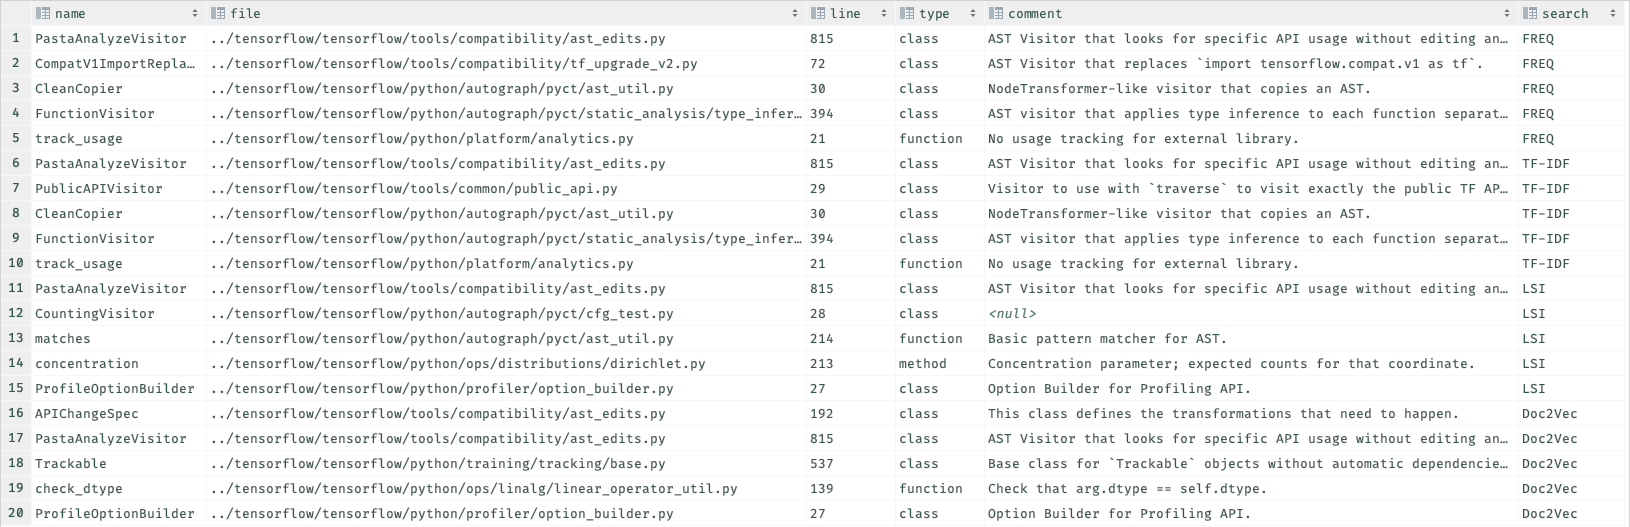
\includegraphics[width=0.95\textwidth]{../res/part2.png}
\caption{Results of the given query}\label{fig:Part2}
\end{figure}


\section{Evaluation of search engines} % 3
\subsection{Goal and Input parameter} % 3: goal & input
This part of the project consists of measuring the precision and recall given 10 queries along with their ground truth.\\
This file takes as argument the path of the ground truth file.

\subsection{Description of the code} % 3: code description
The function \texttt{start(path\_ground\_truth)} loads the csv of the data  into a pandas dataframe, parses the ground truth and then computes the precision and recall.\\
To efficiently parse the ground truth file, we created a class named \texttt{Truth} which holds the name, path and query. We read the ground truth file and create an array with all the entries of the ground truth and the queries.\\
To compute precision and recall we get the data of the results and the embedding vectors from the previous part. We create a dictionary to save the scores of the queries and a dictionary for the vectors. We then compute the precision and recall, by comparing our results and the ground truth.

\subsection{Results} % 3: comment results
Table \ref{tab:Evaluation} show the statistics of precision and recall compared to the ground truth.
We can see that the precision is low for all engines. The engine with the highest precision is \texttt{Doc2Vec}. 
The recall is higher than the precision. The engine \texttt{TF-IDF} has a recall equal to $1$. The second highest recall is of \texttt{Frequencies} with score $0.9$. Both \texttt{LSI} and \texttt{Doc2Vec} have a recall of $0.8$.

\begin{table}[h]
\centering
\begin{tabular}{| l r r |}
\hline
\textbf{Engine}	&  \textbf{Precision}	&  \textbf{Recall}	\\ \hline\hline
Frequencies 		&	0.332	&	0.9	\\
TD-IDF			&	0.365	&	1.0	\\
LSI				&	0.403	&	0.8	\\
Doc2Vec			&	0.417	&	0.8	\\ \hline
\end{tabular}
\captionof{table}{Statistics of the search engines}\label{tab:Evaluation}
\end{table}


\section{Visualisation of query results} % 4
\subsection{Goal and Input parameter} % 4: goal & input
This part of the project consists of visualizing the embedding vectors of the queries and the top 5 answers in a 2D plot.
This file takes as argument the ground truth file.

\subsection{Description of the code} % 4: code description
The first part of the execution is the same as the previous file. After the results are calculated, we plot the TSNE of the embedding vectors, that we retrieved in the explxanation above but we did not use. The plot is straight-forward: we create a dataframe with the information of x and y coordinates and print them of different hues.
\subsection{Results} % TODO 4: comment results
Figure \ref{fig:plots} shows the plots of the visualization of the queries.

\begin{figure}[h]
\centering
\begin{subfigure}[t]{0.45\textwidth}
\centering
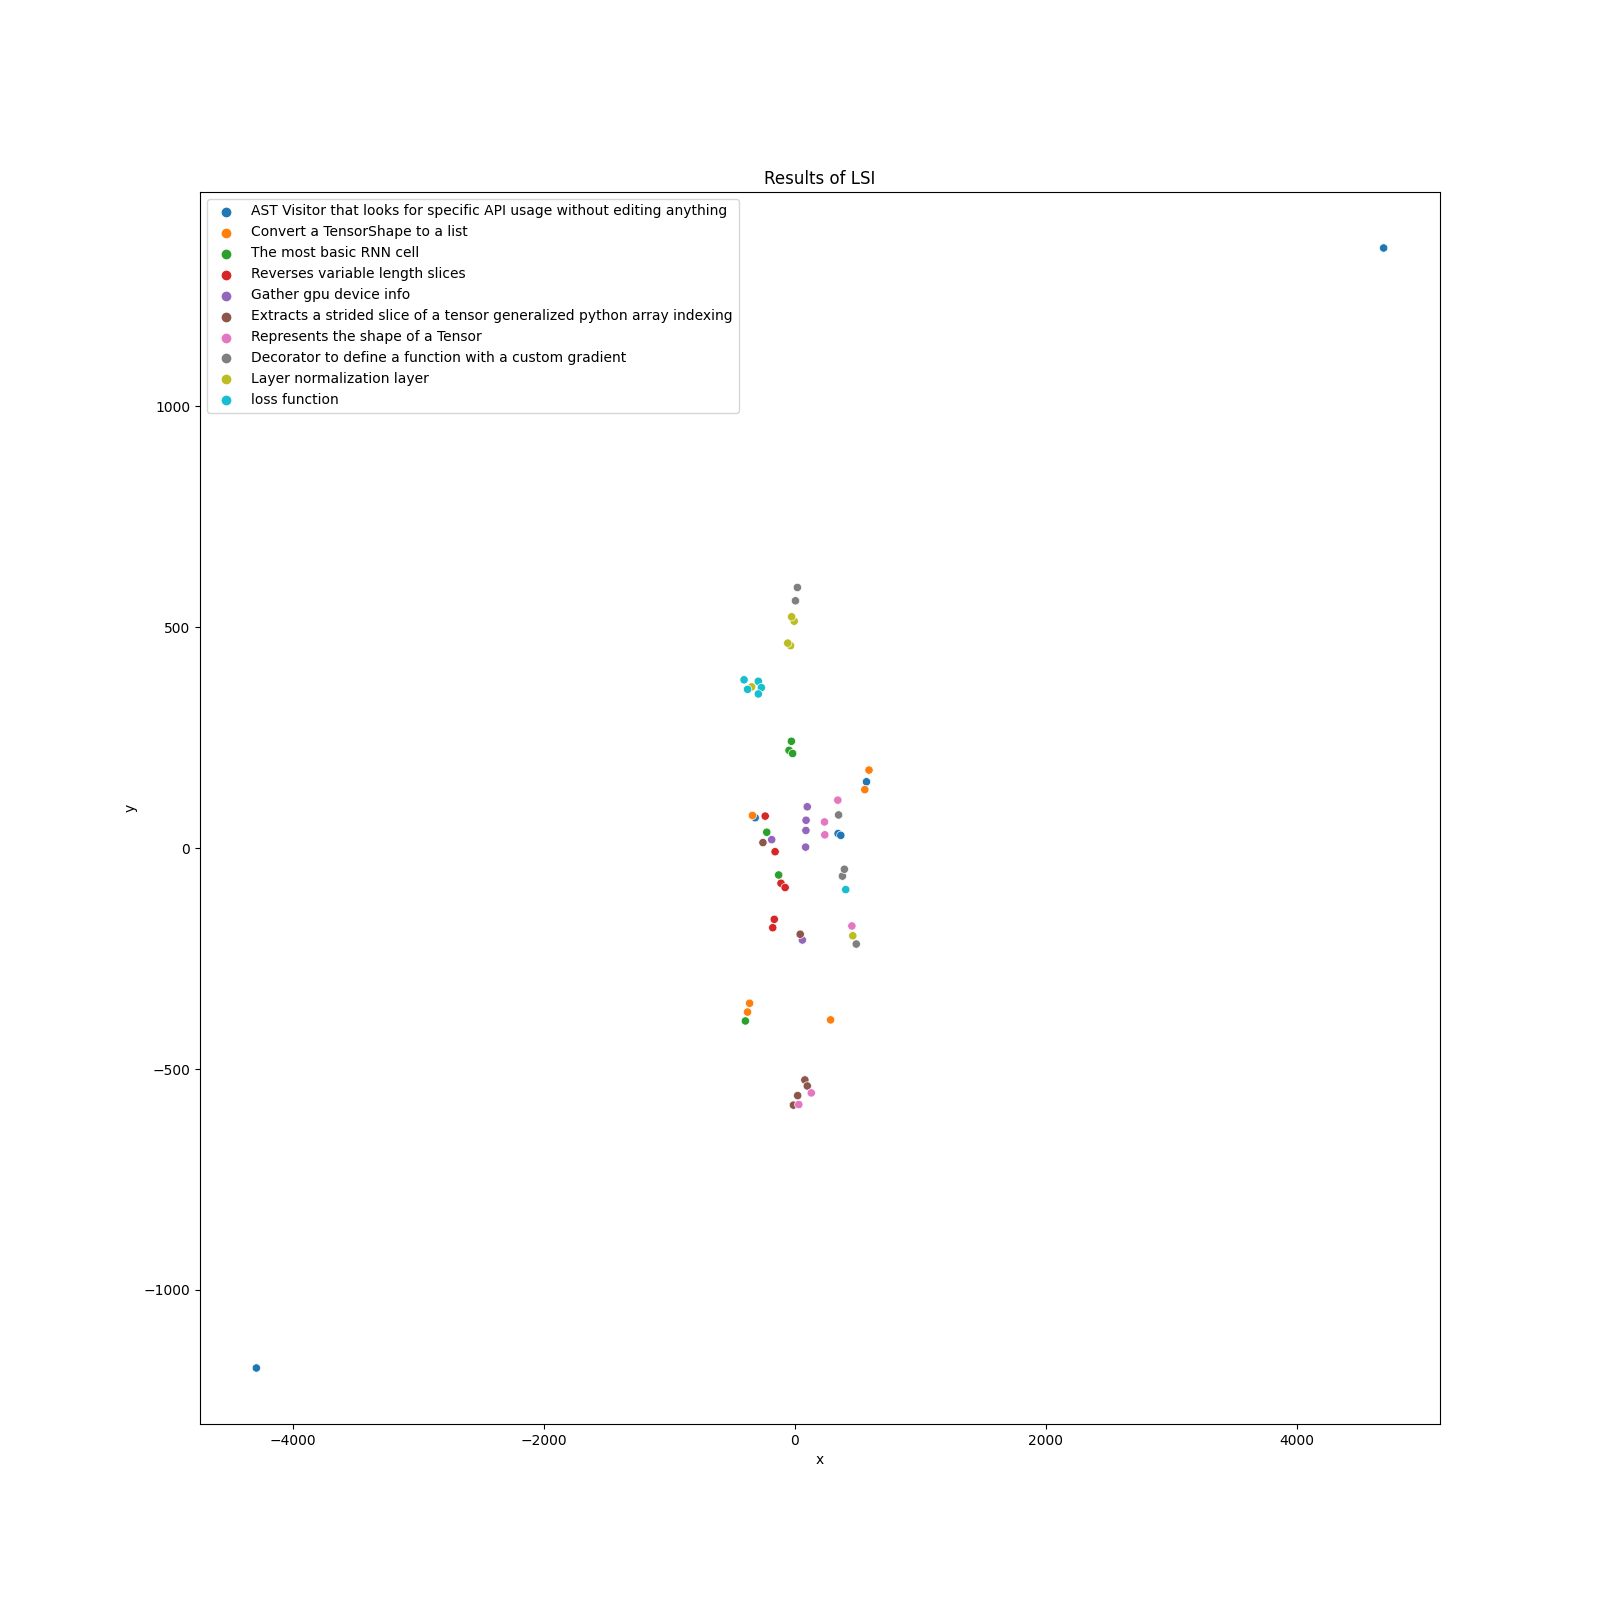
\includegraphics[width=\textwidth]{../res/lsi.png}
\caption{Results of LSI}\label{fig:lsi}
\end{subfigure}
\hfil
\begin{subfigure}[t]{0.45\textwidth}
\centering
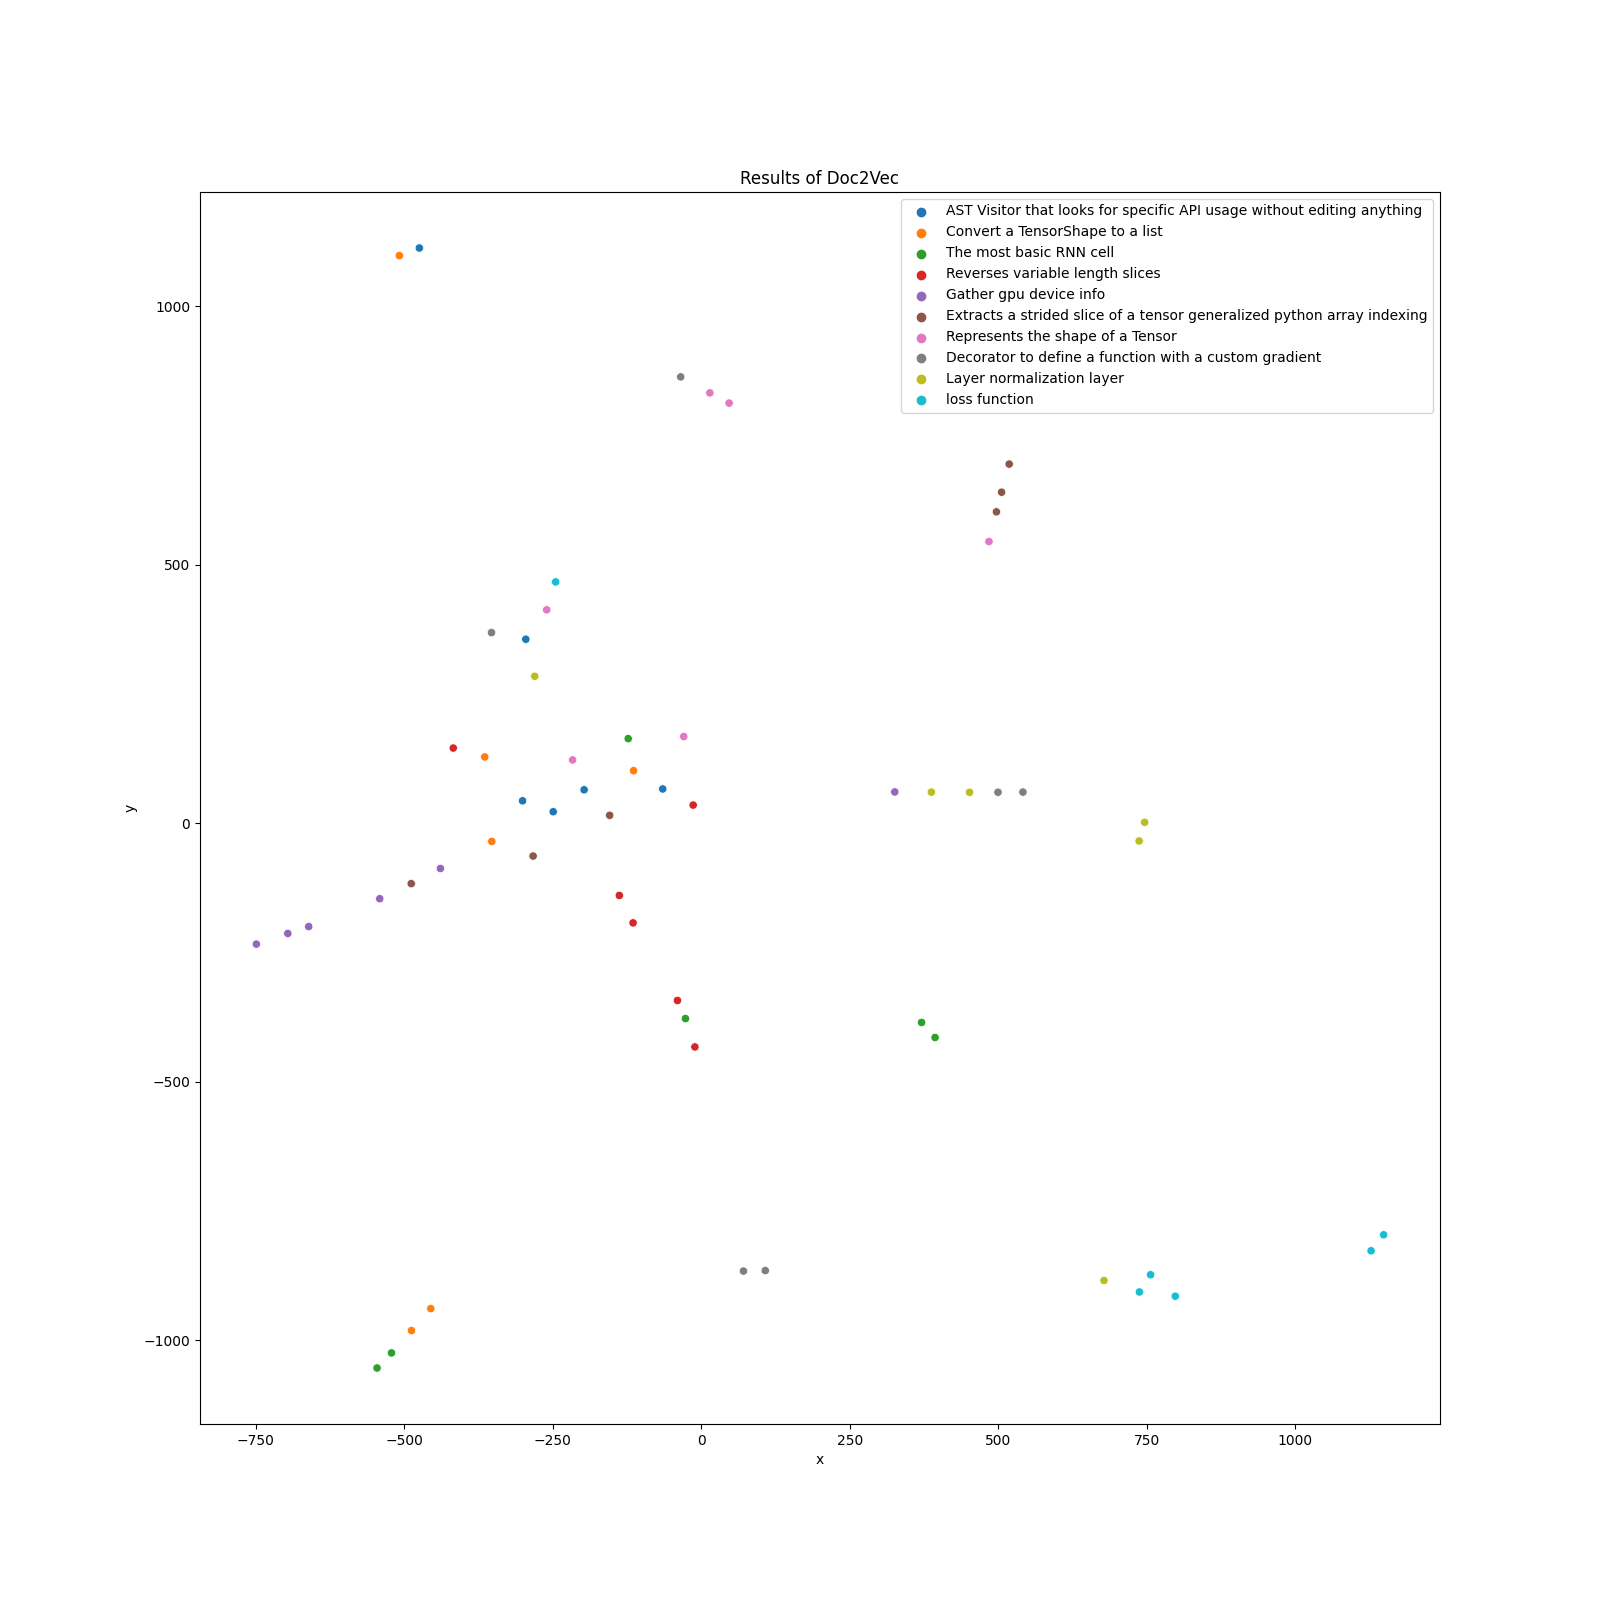
\includegraphics[width=\textwidth]{../res/doc2vec.png}
\caption{Results of Doc2Vec}\label{fig:doc2vec}
\end{subfigure}
\caption{Visualization of the plots of the queries}
\label{fig:plots}
\end{figure}

\newpage
\appendix

\section{Python code}

\subsection{Data Extraction}
\lstinputlisting{../src/extract_data.py}
\subsection{Training of search engines}
\lstinputlisting{../src/search_data.py}
\subsection{Evaluation of search engines and Visualisation of query results}
\lstinputlisting{../src/prec_recall.py}


\section{Bash Code} 
\lstinputlisting[language=Bash]{../run.sh}

\end{document}